\documentclass[UTF8, a4paper, linespread=1.5]{article}

\usepackage{tcolorbox, listings, algorithm, minted, algpseudocode}
\usepackage{geometry, savesym, amsmath, enumerate, indentfirst, color, amsthm, bm, extarrows, ulem}
\usepackage{amssymb}
\usepackage{nameref, hyperref}
 \geometry{top=3cm, bottom=3cm, left=1.5cm, right=1.5cm}

\usepackage{enumitem}
\setenumerate[1]{itemsep=0pt,partopsep=0pt,parsep=\parskip,topsep=5pt}
\setitemize[1]{itemsep=0pt,partopsep=0pt,parsep=\parskip,topsep=5pt}

\renewcommand\contentsname{Contents}

\tcbuselibrary{skins, breakable, theorems}

% \setlength{\leftskip}{10pt}
\setlength{\parindent}{10pt}
% \setlength{\parskip}{2em}
\renewcommand{\baselinestretch}{1.3}

\newcounter{RomanNumber}
\newcommand{\mrm}[1]{(\setcounter{RomanNumber}{#1}\Roman{RomanNumber})}

\newtcbtheorem{thm}{}
  {enhanced, theorem name and number, code={\edef\@currentlabelname{#2}}, 
  frame code={
        % \path[thick, draw] (frame.north west) -| (frame.north east) -| (frame.south east) -| (frame.south west) -| (frame.north west);
        \path[thick, draw] (frame.north west)  +(.5\baselineskip,0) -| +(0,-.5\baselineskip);
        % \path[thick, draw] (frame.north east) +(-.5\baselineskip,0) -| +(0,-.5\baselineskip);
        % \path[thick, draw] (frame.south west) +(.5\baselineskip,0) -| +(0,.5\baselineskip);
        \path[thick, draw] (frame.south east) +(-.5\baselineskip,0) -| +(0,.5\baselineskip);
    },
    left=1mm, right=1mm, top=1mm, bottom=1mm,
    colback=black!5,
    colframe=red!75!black,
    colbacktitle=black!0,
    coltitle=black!100,
    fonttitle=\bfseries}{thm}


\usepackage{environ}
\RenewEnviron{math}{%
\begin{align*}
\BODY
\end{align*}
}

\title{CS217 -- Algorithm Design and Analysis \\ Homework 5}
\date{\today}
\author{Not Strong Enough}



\begin{document}

    \maketitle

    \begin{thm}{}{}
        Let $\nu(G)$ denote the size of a maximum matching of $G$.
        Obviously, ${\rm val}({\rm MLP}(G))\ge \nu(G)$ for all graphs.
        Show that $\nu(G)={\rm val}({\rm MLP}(G))$ for all bipartite graphs $G$.
        Do this without referring to K\H{o}nig's Theorem.
    \end{thm}
    \begin{proof}[Solution]
        Suppose $\mathbf{x}$ is a solution to MLP$(G)$.
        $E_F$ is the set of edges with fractional values in $\mathbf{x}$.
        First do as follows:
        \begin{itemize}
            \item[(1)] If $E_F$ doesn't contain a cycle, terminate.
            \item[(2)] Find a cycle in $E_F$ with fractional values, denote it $C:=\{e_i\in E_F :1\le i \le n,i\in\mathbb{N}\}$.
            \item[(3)] Add $x_{e_{2k-1}}$ by $\epsilon$ and $x_{e_{2k}}$ by $-\epsilon$ for $\{k\in \mathbb{N}:k \le n/2\}$.
            \item[(4)] Increase $\epsilon$ until there exists $i$ such that $x_{e_i}=0 \text{ or } 1$.
            \item[(5)] go to step(2) if there exists a cycle in $E_F$.
        \end{itemize}
        Since $G$ is a bipartite, $C$ can only be a even cycle, so step (3) makes sense.
        If we modify the solution by step(3), obviously the constraints of MLP$(G)$ will still be satisfied, and the target function will remain unchanged.
        The process will terminate because $|E_F|$ decreases by at least 1 in each iteration.

        Then do as follows:
        \begin{itemize}
            \item[(1)] If $E_F$ is empty, terminate.
            \item[(2)] Choose 2 vertex $v_1,v_2$ that $|\{x_e\in(0,1):v_1\in e\}|=1$, $|\{x_e\in(0,1):v_2\in e\}|=1$ and there's a path between $v_1$ and $v_2$ in $E_F$, denote it $P:=\{e_{i}'\in E_F:1\le i \le m,i\in\mathbb{N}\}$
            \item[(3)] Add $x_{e_{2k-1}'}$ by $\epsilon$ for $\{k\in\mathbb{N}:2k-1\le m\}$ and $x_{e_{2k}'}$ by $-\epsilon$ for $\{k\in\mathbb{N}:2k\le m\}$
            \item[(4)] Increase $\epsilon$ until there exists $i$ such that $x_{e_{i}'}=0 \text{ or } 1$
            \item[(5)] Go to step (2) if $E_F$ is not empty
        \end{itemize}
        Since there's no cycle in $E_F$, we can definitely choose $v_1,v_2$ that satisfy the requirements if $E_F$ is not empty.
        In each iteration, the target function will not decrease.
        Since $v_1,v_2$ can only be touched by edges with fractional value or value 0, the constraints of $v_1,v_2$ can be satisfied.
        In other words, $\sum_{e\in E:v_1\in e}x_e =x_{e_{1}'} \le 1$, $\sum_{e\in E:v_2\in e}x_e =x_{e_{m}'} \le 1$
        The constraints of other vertices $v$ in $P$ will obviously be maintained.
        The process will termintate because $|E_F|$ decreases by at least 1 in each iteration.

        Finally, after 2 processes, the solution becomes integral and the value of target function does not decrease, which means $\text{ int-val}(MLP(G))\ge {\rm val}(MLP(G))$.
        And we already have  $\text{int-val}(MLP(G))\le {\rm val}(MLP(G))$.
        So $\nu(G)=\text{int-val}(MLP(G))= {\rm val}(MLP(G))$
    \end{proof}

    \newpage

    \begin{thm}{}{}
        We know that $\nu(G) = \tau(G)$ for all bipartite graphs (K\H{o}nig's Theorem) and $\nu(G) \leq \tau(G)$ for all graphs (since every matched edge must be covered by a distinct vertex). Show that $\tau(G) \leq 2\nu(G)$ for all grpahs $G$.
    \end{thm}

    \begin{proof}
        Let $M$ be a maximum matching of $G$. It follows that $|M| = \nu(G)$. Now we choose our vertex set $V'$ to be all the matched vertices in $G$. So $|V'| = 2\nu(G)$. 
        
        Claim that $V'$ is a vertex cover. To see that, assume there exists an edge $(u, v)$ which is not covered by $V'$. It means that neither $u$ nor $v$ is matched. So we can add edge $(u, v)$ to $M$, and thus $M$ is not maximum, which leads to a contradiction.
        
        So the size of minimum vertex cover $\tau(G) \leq |V'| = 2\nu(G)$.
    \end{proof}

    \bigskip

    \begin{thm}{}{}
        Show that $\tau(G) \leq 2{\rm opt}({\rm VCLP}(G))$ for all graphs $G$ (including non-bipartite graphs).
    \end{thm}

    \begin{proof}
        From (2) we know that $\tau(G) \leq 2\nu(G)$. Since $\nu(G) \leq {\rm opt}({\rm MLP}(G)) \leq {\rm opt}({\rm VCLP}(G))$, it follows that $\tau(G) \leq 2\nu(G) \leq 2{\rm opt}({\rm VCLP}(G))$.
    \end{proof}

    \newpage
    
    \begin{thm}{}{}
        For a graph $G = (V, E)$, let $\tau(G)$ denote the size of a minimum vertex cover, and $\nu(G)$ the size of a maximum matching. Recall the two linear programs VCLP and MLP. Let $\tau_f(G) := {\rm opt}({\rm VCLP}(G))$ and $\nu_f(G) := {\rm opt}({\rm MLP}(G))$. Note that
        $$
        \nu(G) \leq \nu_f(G) = \tau_f(G) \leq \tau(G),
        $$
        where the equality in the middle follows from Strong LP Duality. Also, if $G$ is bipartite, then the equality holds throughout in (1). Let us say a graph $G$ is {\it VCLP exact} if $\tau(G) = \tau_f(G)$, and {\it MLP exact} if $\nu(G) = \nu_f(G)$. As we already know, a bipartite grpah $G$ is both VCLP exact and MLP exact.
        
        From now on, suppose that $G$ is {\it not} bipartite but $\tau(G) = \tau_f(G)$.
        
        \begin{enumerate}
            \item Give an example of such a graph $G$ that is not bipartite but still VCLP exact.
            \item Give an example of a graph $G$ that is MLP exact but not VCLP exact.
            \item Suppose $G$ is VCLP exact. Let $Y \subseteq V(G)$ be a minimum vertex cover. Let $\mathbf{x}$ be an optimal solution of MLP($G$). Show that $x_e = 0$ if $e \subseteq Y$ (i.e., if both endpoints of $e$ are in the cover).
            \item Show that such a graph $G$ has a matching of size $|Y|$, and thus is MLP exact, too.
        \end{enumerate}
    \end{thm}

    \begin{center}
        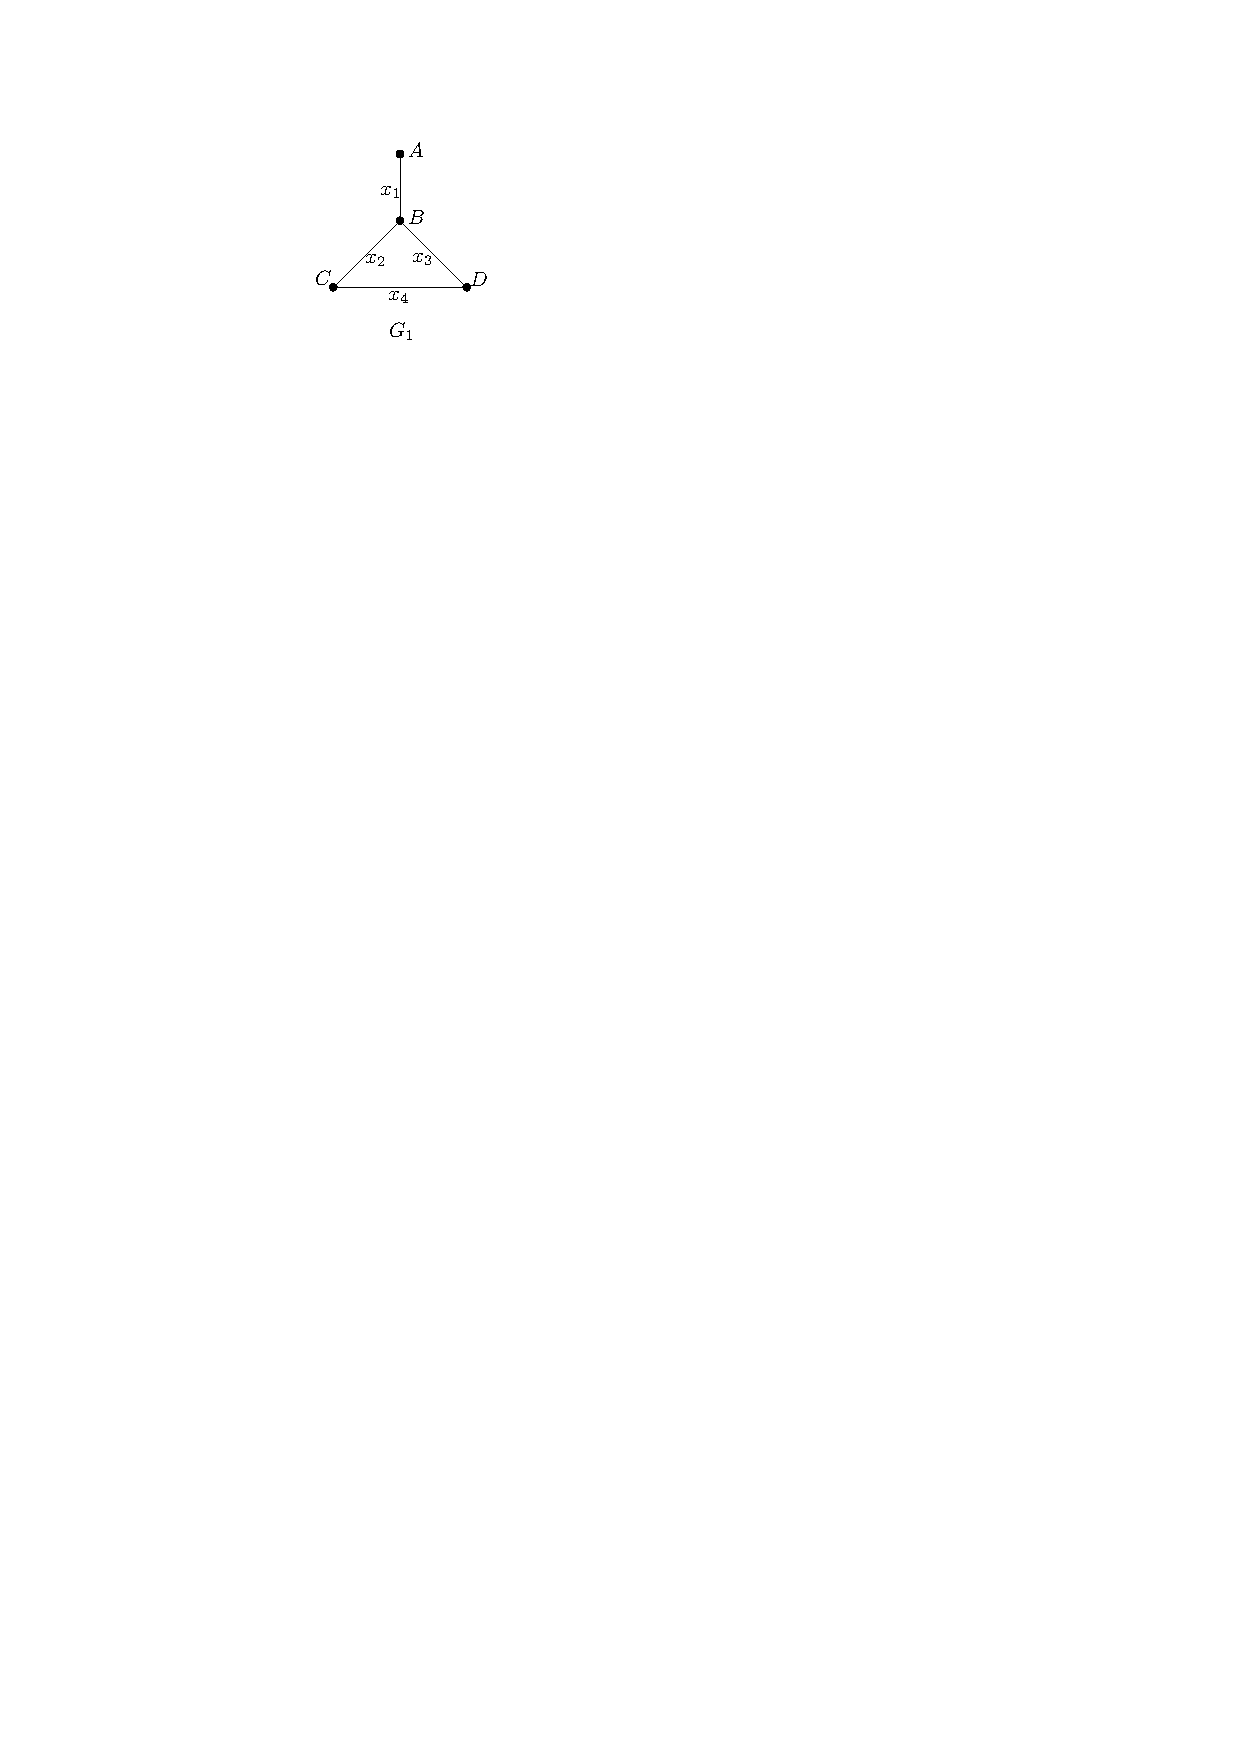
\includegraphics[width=0.16\textwidth]{figure4_1.pdf}
        \hspace{3cm}
        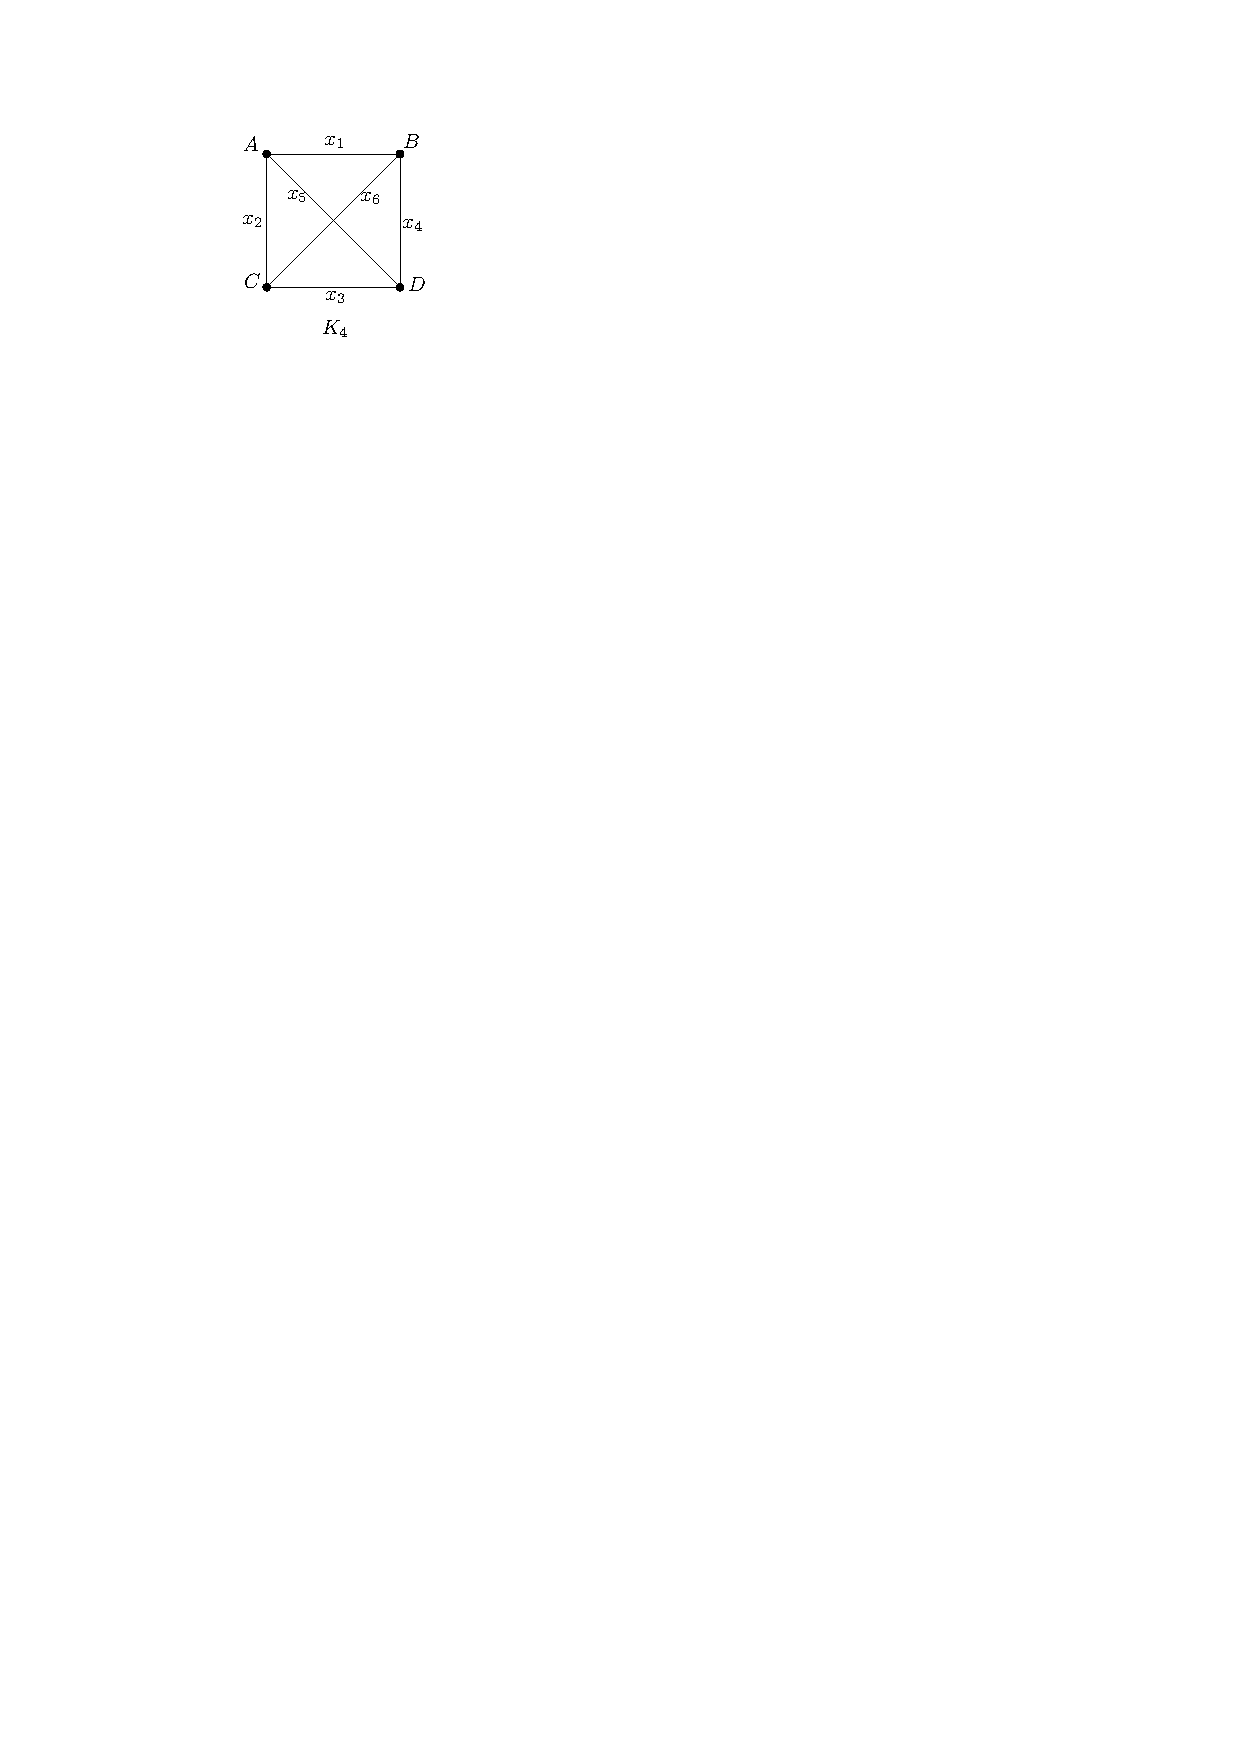
\includegraphics[width=0.16\textwidth]{figure4_2.pdf}
    \end{center}

    \begin{proof}[Solution to (1) and (2).]
        ~
        \begin{enumerate}
            \item The example is $G_1$ in the upper left. It is not bipartite since $B, C, D$ constitute an odd cycle.
            
            The minimum vertex cover of $G_1$ can be $\{B, C\}$ or $\{B, D\}$, with size $2$. So $\tau(G_1) = 2$.
            
            VCLP$(G_1)$ is
            \begin{center}
                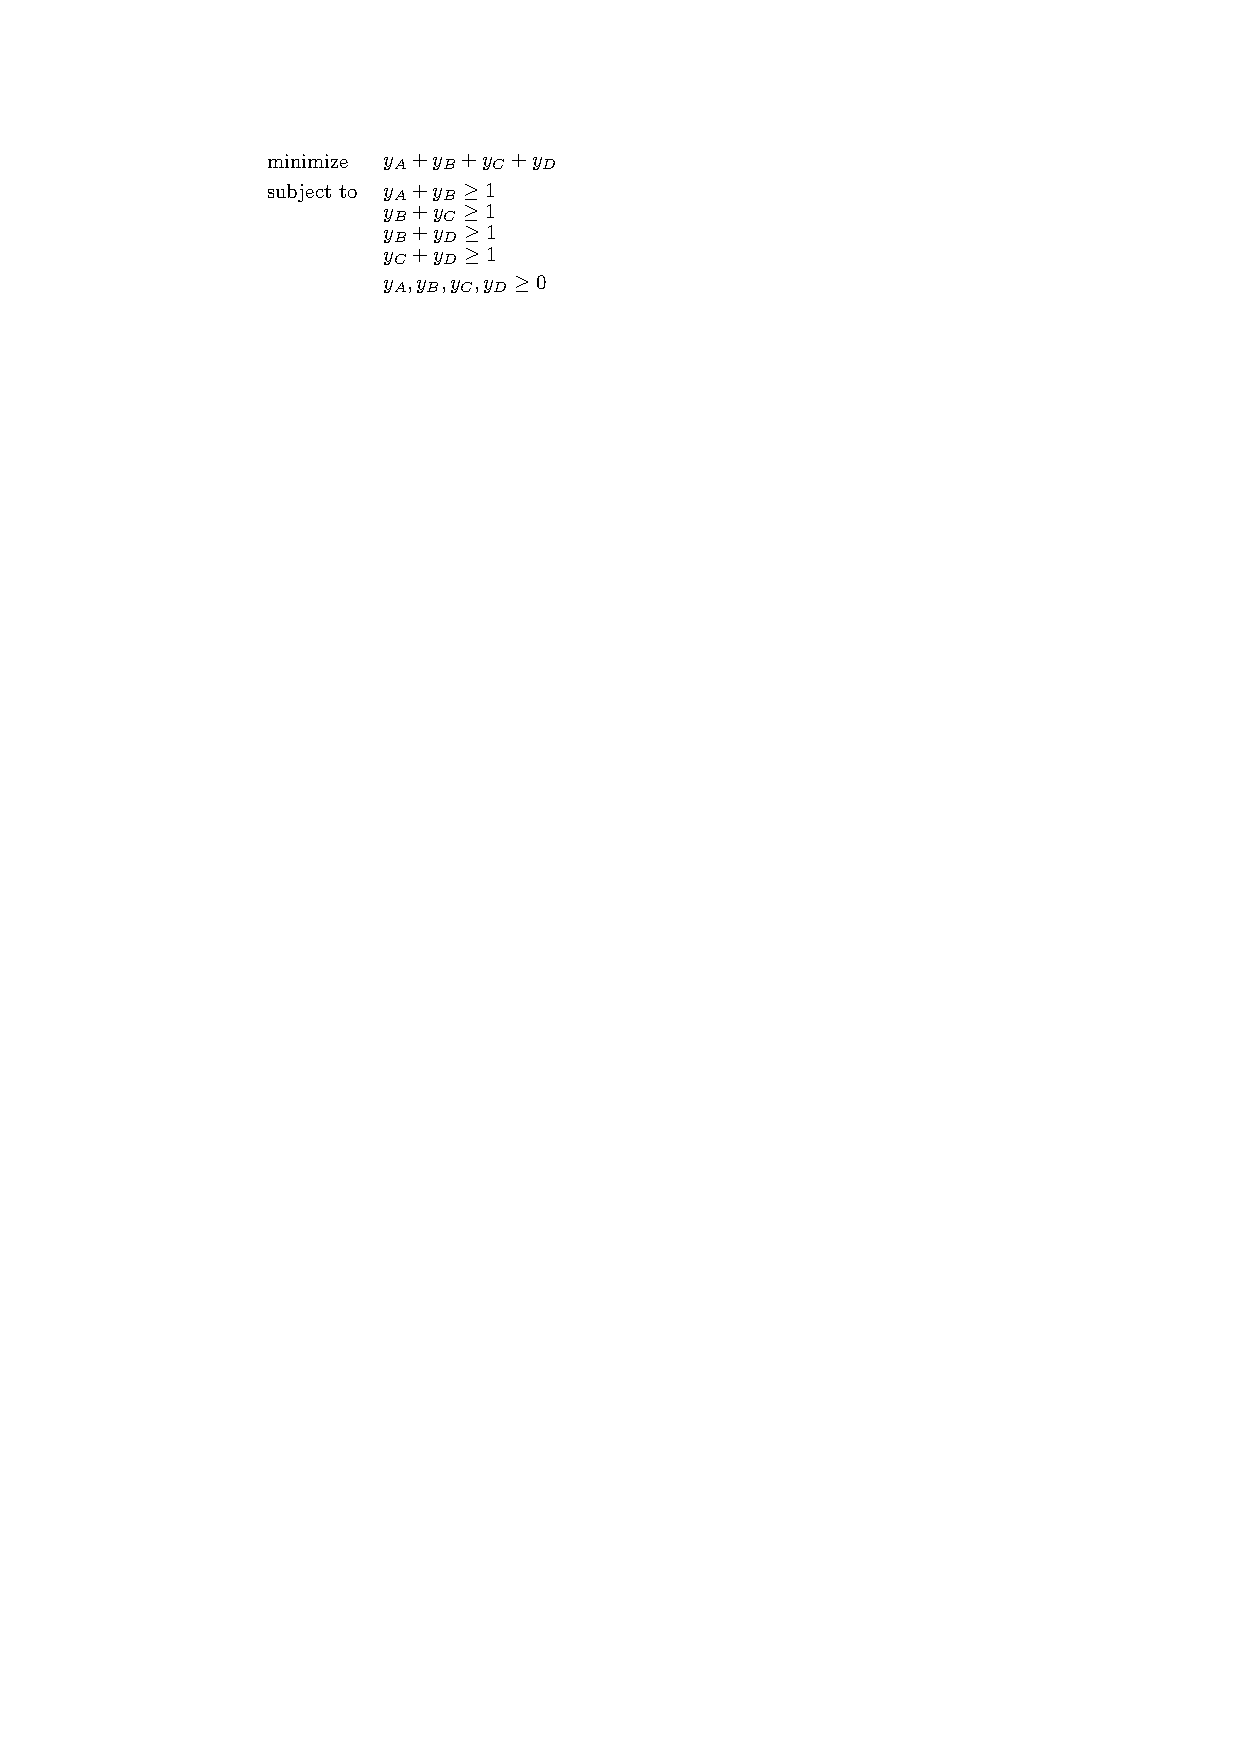
\includegraphics[width=0.28\textwidth]{VCLP4_1.pdf}
            \end{center}
            Note that if we add up the constraints $y_A + y_B \geq 1$ and $y_C + y_D \geq 1$, we get $y_A + y_B + y_C + y_D \geq 2$, which gives a lower bound of the target function.
            
            Since $\tau(G_1) = 2$, it follows that the lower bound is tight. Hence $\tau_f(G_1) = \tau(G_1) = 2$.
            
            So $G_1$ is an example which is not bipartite but still VCLP exact.
            
            \item The example is $K_4$ in the upper right. The minimum vertex cover can be $\{A, B, C\}, \{A, B, D\}, \{A, C, D\}$ and $\{B, C, D\}$, with size $3$. So $\tau(K_4) = 3$.
            
            However, by setting the value of each vertex to $0.5$, we find that all edges are exactly covered ($y_u + y_v = 1$ for edge $(u, v)$). So $\tau_f(K_4) \leq 2$, and thus $K_4$ is not VCLP exact.
            
            Now consider the maximum matching and MLP. Obviously we can only match $2$ pairs of vertices. So $\nu(K_4) = 2$, and $\nu_f(K_4) \geq 2$ follows. Since we already know that $\tau_f(K_4) \leq 2$ and $\nu_f(K_4) = \tau_f(K_4)$ by Strong LP Duality, we can conclude that $\nu(K_4) = \nu_f(K_4) = \tau_f(K_4) = 2$. Therefore $K_4$ is MLP exact.
            
            So $K_4$ is an example which is MLP exact but not VCLP exact.
  
            In (3) and (4), suppose that $Y$ is a minimum vertex cover of $G$. Note that there is no edge $(u, v) \in E$ such that both $u, v \in V \setminus Y$. Because $u, v \in V \setminus Y$ means that $(u, v)$ is not covered by $Y$, which is contradict with $Y$ being a vertex cover.

            \item VCLP is to minimize $c^Ty$ with constraints $A\cdot y\geq b$, and MLP is to maximize $b^Tx$ with constraints $A^Tx\leq c$, where $b=1,c=1$. 
            
            So there is $$x^T \cdot b \leq x^T \cdot A \cdot y \leq c^T \cdot y$$

            By strong duality, let optimal solution be $x^{(0)},y^{(0)}$, there is $b^T * x^{(0)} = c^T * y^{(0)}$
            
            Let $A \cdot y^{(0)}=b^{(0)}$,there is $(b^T - b_0^T)\cdot x_0=0$. As $A\cdot y >= b$, there is $b_e-b^{(0)}_e\leq 0,\forall e\in E$. Besides, there is $x^{(0)}_e\geq 0,\forall e\in E$. 
            
            So if $b^T_e-b^{(0)}_e<0$,there is $x^{(0)}_e=0$. 

            Let $y^{(0)}$ be the solution corresponding to the vertex cover(by VCLP exact, it is an optimal solution of VCLP), then there is 
            $b_e-b^{(0)}_e=1-2<0,\forall e\in Y$, so $x^{(0)}_e=0,\forall e\in Y$ for each optimal solution $x^{(0)}$ of the MLP. 
            
            \item Define $N(\cdot)$ be: 
            $$N(A)=\{v:v\text{ is the neighbor of some }u\in A\}\cap (V \setminus Y)$$
            We claim that if $A\subseteq Y$, then $|A|\leq |N(A)|$. 

            Otherwise, if $A\subseteq Y$ and there is $|B|<|A|$ where $B=N(A)$. 

            Consider an optimal solution of VCLP relative to $Y$(that is, if $v\in Y$, $y_v=1$, otherwise $y_v=0$). Let 
            \begin{equation*}
                y_v'=
                \begin{cases}
                    y_v-\epsilon&,v\in A\\
                    y_v+\epsilon&,v\in B\\
                    y_v &,\text{ otherwise. }
                \end{cases}
            \end{equation*}
            where $\epsilon < \frac{1}{2}$. For edge $(u, v) \in E$: 
    
            a) $y_u'+y_v'\geq 1$ for $u,v\in A$. Since there is $y_u'+y_v'= (1-\epsilon)+(1-\epsilon)=2-2\epsilon>1$; 
            
            b) $y_u' + y_v' \geq 1$ for $u \in A, v \in Y \setminus A$. Since there is $y_u' + y_v' = (1 - \epsilon) + 1 = 2 - \epsilon > 1$;
    
            c) $y_u'+y_v'\geq 1$ for $u\in A, v\in B$. Since there is $y_u'+y_v' = (1-\epsilon) + \epsilon=1$;
            
            d) $y_u' + y_v' \geq 1$ for $u \in Y \setminus A, v \in B$. Since there is $y_u' + y_v' = 1 + \epsilon > 1$;
    
            e) The rest of constraints remains holding since the left hand side is not changed from solution $(y_v)$. 
    
            So $(y_v)'$ is a solution to the VCLP, too. But it is $\epsilon(|A|-|B|)$ less than solution $(y_v)$, which rises a contradiction that $Y$ is a minimum solution. 
        
            Hence what we claimed is proved. Remove all edges from $Y$ to $Y$, the graph is a bipartite graph $G$ with $L = Y$, $R = V\backslash Y$. By what we claimed, there is $|L|\leq|R|$

            Notice that what we claimed exactly means that the condition of Hall's Theorem is satisfied, so by Hall's Theorem, there is a perfect matching of size $|L|=|Y|$. 
        \end{enumerate}
    \end{proof}
\end{document}

